\documentclass[11pt,letterpaper]{article}
\usepackage[T1]{fontenc}
\usepackage{lmodern,microtype}
\usepackage[margin=0.94in,top=0.86in,bottom=0.86in]{geometry}
\usepackage{amsmath,amssymb,amsthm,mathtools}
\usepackage{graphicx,booktabs,tabularx,array,enumitem,xcolor,fancyhdr}
\usepackage[hyphens]{url}
\usepackage[colorlinks=true,linkcolor=linkblue,urlcolor=linkblue,citecolor=linkblue,bookmarksnumbered]{hyperref}
\usepackage{bookmark}
\definecolor{linkblue}{HTML}{1D5269}
\definecolor{ink}{HTML}{173747}
\usepackage{titlesec}
\titleformat{\section}{\Large\bfseries\color{ink}}{\thesection}{0.65em}{}
\titleformat{\subsection}{\large\bfseries\color{ink}}{\thesubsection}{0.6em}{}
\setcounter{tocdepth}{1}
\newtheorem{theorem}{Theorem}[section]
\newtheorem{lemma}[theorem]{Lemma}
\newtheorem{proposition}[theorem]{Proposition}
\newtheorem{corollary}[theorem]{Corollary}
\theoremstyle{definition}
\newtheorem{definition}[theorem]{Definition}
\newtheorem{example}[theorem]{Example}
\newtheorem{remark}[theorem]{Remark}
\newcolumntype{Y}{>{\raggedright\arraybackslash}X}
\setlist{nosep,topsep=5pt}
\setlength{\emergencystretch}{2.5em}
\pagestyle{fancy}\fancyhf{}\fancyhead[L]{\small\textcolor{linkblue}{Finite observations in iPRA}}\fancyhead[R]{\small\thepage}
\setlength{\headheight}{15pt}\renewcommand{\headrulewidth}{0.3pt}
\hypersetup{pdftitle={From oracle observations to iPRA proofs},pdfauthor={Research report prepared for Vladimir Reshetnikov}}
\newcommand{\Prf}{\mathsf{Prf}\,\mathsf{PRAAx}}
\newcommand{\PL}{\mathrm{PL}}
\newcommand{\epsi}[1]{2^{-#1}}
\begin{document}
\thispagestyle{empty}
\noindent{\small\sffamily\bfseries\color{linkblue} CONSTRUCTIVE AND COMPUTABLE ANALYSIS \hfill 20 NOVEMBER 2026}\par
\vspace{1.1em}
\noindent{\Huge\bfseries\color{ink} From oracle observations\\[3pt] to iPRA proofs}\par
\vspace{0.7em}
\noindent{\large Finite information for roots, derivatives, and probability laws}\par
\vspace{1em}
\noindent A theorem about a continuous object can often be stated as a family of rational
experiments. For each requested precision, which questions must the experiment
ask, how long can it run, and what numerical certificate makes two valid runs
compatible? This report answers those questions for three different operators.
All three accept inexact observations. The proofs identify the data that permit
an arithmetical construction and give examples where weaker data lose the
claimed conclusion.
\medskip

\noindent\begin{tabularx}{\linewidth}{@{}p{0.22\linewidth}Y@{}}
\toprule
Problem & Construction and quantitative result\\
\midrule
Root selection & A lower separation modulus makes one midpoint observation sufficient to halve a sign bracket, even when the observed sign is ambiguous.\\[3pt]
Differentiation & Bounds on adjacent dyadic slopes and a summable tail construct the derivative from values. This supplies the local estimate used to pass to a fundamental theorem of calculus.\\[3pt]
Probability laws & Cumulative piecewise-linear probes recover a transport-Cauchy name for a positive expectation functional on the unit interval. Finite marginals determine sparse optimal couplings, with a proof of optimality.\\
\bottomrule
\end{tabularx}

\medskip
The common interface is finite replay with a numerical use bound, plus a
separate proof of independence of names. The package includes Lean proofs in
the ambient type theory and object-calculus derivations for sparse replay, the midpoint rule, dyadic slope refinement,
and prefix repair. The final section specifies the remaining embeddings.
\tableofcontents
\clearpage
\section{The arithmetic interpretation}
\label{sec:basis}

\subsection{What a presentation means}

Use the repository's ordinary intuitionistic primitive recursive arithmetic.
The only object sort is the natural numbers. Each fixed primitive recursive
(PR) definition has its own symbol. The proof calculus admits first-order
intuitionistic deductions and induction on quantifier-free formulas. In the Lean
implementation the symbols are \texttt{PR k}, terms are \texttt{PTm n}, and the
judgment with assumptions $\Gamma$ and conclusion $A$ is \texttt{Prf PRAAx}
$\Gamma\ A$. Here $n$ counts free numerical variables. We give schemata in fixed
PR algorithms, allowing their numerical parameters, including finite tables, to
vary. A schema can be instantiated by substituting terms and the corresponding
correctness derivations. Its quantification over algorithms belongs to the
metatheory.

A rational can be a signed numerator and a positive denominator. For a total
natural coding, represent the integer numerator by a difference of naturals and
the denominator by one plus a natural. Equality and order are cross-products;
an unreduced fraction is a valid result. Encode finite lists by length and
contents, or use the explicit coding in Section~\ref{sec:oracle}. Each
operation used below has a PR loop bound. One may use the same finite integer
kernel for real, vector, and table observations. Fixed finite product distances
can use the maximum of coordinate distances.

In a rational pseudometric basis $(D,d)$ let $e_p=2^{-p}$. A name is a family
$x_p$ satisfying $d(x_p,x_q)\le e_p+e_q$. Equality of two names means
$d(x_p,y_q)\le e_p+e_q$ at all $p,q$. This definition only needs basis distances,
not a prior construction of an infinite sequence as a set inside arithmetic.
For fixed PR families these are first-order formulas. Externally the same
conditions describe arbitrary Cauchy names in the completion. A bound
$|x-r|\le b$ for a named scalar and a rational means
$|x_p-r|\le b+e_p$ for every $p$. Sums, rational multiples and order inequalities
of named scalars are read with the sum of the individual absolute error bounds.
This convention also applies to the $F(q)$ and $L(f)$ notation below.

An elementary rule removes auxiliary precision parameters. Suppose rational
$A,B$ satisfy $A\le B+c2^{-r}$ for every $r$, where $c\ge0$ is a supplied
rational. If $A>B$, the positive difference has an explicitly positive
numerator. With $A-B=a/d$ and $c=b/s$, choose, for instance, $r=bd+1$;
then $2^r>bd$ and $c2^{-r}<a/d$. Decidable rational order gives $A\le B$.
All products and powers are PR. This allows calculations with named scalars to
be expanded into rational inequalities one observed precision at a time.

\subsection{A rule for transferring estimates}

\begin{theorem}[Two-run error rule]\label{thm:tworuns}
Suppose the stage-$p$ algorithm returns a basis element $v$ and a finite
transcript. There is a PR producer on the admitted numerical inputs. Assume
that from any two valid transcripts at stages $p,q$ on compatible inputs one
can derive
\[
                          d(v,w)\le e_p+e_q.
\]
Then the stage algorithm names an output point, and equivalent inputs have
equivalent outputs. If two proposed regular names $y,z$ satisfy
$d(y_i,v_k)\le e_i+\rho(k)$ and $d(z_j,v_k)\le e_j+\sigma(k)$ for all
$i,j,k$, with a supplied schedule $k(t)$ such that
$\rho(k(t))+\sigma(k(t))\le e_t$, then $y$ and $z$ are equal as names.
\end{theorem}
\begin{proof}
Use the two-run inequality on the same input, at two precisions, to get
regularity. Apply it to two names of the same input to get extensionality.
For uniqueness fix one precision of each of the two proposed outputs. Compare
both to an arbitrarily fine observation of the produced point. Add the
two bounds by the triangle inequality, then eliminate the surplus term with
the preceding rational rule. Each use instantiates a universal numerical
hypothesis. There is no selection of infinitely many witnesses.
\end{proof}

One common way of proving the two-run hypothesis is to compare each run to
the same rational test functional with error $e_p$. In the law construction
the distinguishing test is itself produced from the two finite outputs.
In the root construction one compares rational brackets before estimating
a residual. A checker which accepts candidate observations supplies a soundness
implication. To obtain the theorem's producer one must also give the candidate,
an explicit bounded search with a proved success premise, or a PR iteration
with a proved terminal condition.

A finite proof that uses a loop should state its invariant at a fixed final
precision. For a comparison needed at every $i<N$, a bounded conjunction is
compiled as the product of Boolean comparisons, or as the test that the sum of
failure bits is zero. The induction formula is an equation of terms. A universal
contract may be held as a hypothesis and instantiated at a computed index
inside a step. Inducting directly on a universal statement about all functions,
all levels, or all future inputs would require a different rule.

\subsection{Relation to the ProveIt packets}

The development uses revision \texttt{b2341af5370c} of ProveIt. Its
finite-query normal form already codes a bounded finite path, and its continuous
frameworks already give completion, effective compactness and residual-to-name
rules. Our use of finite observations builds on those results. Three more
specific comparisons determine the applications.

\begin{itemize}
\item The analysis library has polynomial bisection, root names and uniqueness
results. Section~\ref{sec:conditioned-zero} asks what comparison at a midpoint can
be replaced by when only a noisy observation of a general function is available.
\item The calculus packet proves FTC II assuming derivative information.
\texttt{TaggedFTC} proves the summation of upper and lower cell estimates.
Section~\ref{sec:dyadicapplication} constructs derivative information from a
condition on the value tables, including behavior at old grid knots.
\item The expected-value packet defines a simple-law name using finite
couplings as data. Section~\ref{sec:laws} produces such couplings from
marginal tables on the line and, one step earlier, produces the marginal
tables from an oracle for expectations of continuous polygonal probes.
\end{itemize}
Revision-specific links and reproduction instructions appear in the final
section and in the source inventory in the archive.

\section{Finite oracle observations and the computability boundary}
\label{sec:oracle}

A realizer in Type-2 computable analysis receives a \emph{name} of an input.
The name can be an arbitrary infinite sequence, even when the realizer is a
computable machine. Two names of the same point can give different finite
answers. These two facts determine what a translation into first-order arithmetic
must preserve. We use the represented-space interpretation of Pauly and distinguish
the number of queries from the cost of reading and processing answers as in
Kawamura and Cook.\footnote{A. Pauly, \emph{On the topological aspects of the
theory of represented spaces}, \url{https://arxiv.org/abs/1204.3763}.
A. Kawamura and S. Cook, \emph{Complexity theory for operators in analysis},
\url{https://arxiv.org/abs/1305.0453}.}

\subsection{Compiling finite use into first-order arithmetic}

Fix five primitive recursive (PR) maps $I(n),q(s),D(s,v),E(s),R(n)$.
They initialize a state, give its next query index, update it on an answer,
extract the final output, and count answer slots. Precision, presentation
parameters and read-only rational bounds can be paired into the input.
The external semantics on an oracle $a:\mathbb N\to\mathbb N$ is
\[
  s_0=I(n),\qquad j_i=q(s_i),\qquad s_{i+1}=D(s_i,a(j_i)),\qquad
  F(a)(n)=E(s_{R(n)}).
\]
An early return can store its output in an absorbing state which requests
index zero in any remaining slots. Allow a window of at least one when using
this convention. For a finite word $w$, let $\widehat w$ give its entries at
indices below $|w|$ and zero elsewhere. Write $s_i(w)$ for the run on
$\widehat w$. The function $(n,i,w)\mapsto s_i(w)$ is PR by ordinary
primitive recursion. One can use any PR sequence coding with empty word,
append, length and lookup. For example encode a cons cell $(h,t)$ by
$2^h(2t+1)$ and the empty list by zero; extracting an entry uses the
bounded $2$-adic valuation and iteration of the tail map. Length is obtained
by bounded iteration since the tail of a positive code is smaller.

Let $U(n)$ be a PR number of entries. The following obligation contains only
natural-number quantifiers, and its matrix with the $i$-quantifier bounded
can be evaluated by primitive recursion:
\begin{equation}
 |w|=U(n)\quad\Longrightarrow\quad
 \forall i<R(n)\quad q(s_i(w))<U(n).
 \label{eq:tableguard}
\end{equation}
The obligation is universally closed over $n,w$. It may also be used with
fixed size parameters and with explicitly specified admissible windows. All
unqualified statements below use the displayed all-word version.

\begin{theorem}[Finite replay and window certification]
If two oracles agree on the queries made by the first run through $t$ slots,
the two states at time $t$ agree. Condition~\eqref{eq:tableguard} is equivalent,
in the external semantics, to the same query bound for every infinite oracle.
Consequently a word of length $U(n)$ taken from any name suffices to compute
$F(a)(n)$. For two finite words these replay implications are iPRA theorems.
\end{theorem}
\begin{proof}
Initially the states agree. Equality of the states at slot $i$ makes the
query indices equal. The assumed agreement on that query then makes the
updates equal. In the arithmetic instance, fix the two words and $t$ as
parameters; induction on the forward state equality under the hypothesis
of agreement on the first $t$ queries uses a quantifier-free invariant
(equivalently use $i\le t\Rightarrow s_i=s_i'$). The agreement test is a
bounded Boolean fold.

Given $a$, form its initial word $w$ of length $U(n)$ externally. Apply
the first assertion with $\widehat w$ as the \emph{first} run. By
\eqref{eq:tableguard}, each of its requests lands in $w$ and receives
the same answer from $a$. The states coincide through every slot and all
query indices of $a$ are therefore bounded. In the converse direction use
the oracle $\widehat w$ in the all-oracle assertion. In iPRA a fixed PR
input name $a(p,j)$ supplies the word by a bounded tabulation in the
parameters $p,n$; arbitrary external names never have to be coded by single
natural numbers.
\end{proof}

The same proof validates a sparse transcript. To check an alleged list of
pairs $(j_i,v_i)$, recompute each state, check $j_i=q(s_i)$, and check
$v_i=v_k$ for every earlier $k$ whose query equals $j_i$. On a supplied
word also check each value against its lookup. All these tests are bounded.
A consistent transcript by itself has an extension as a Baire name: use its
recorded values on queried indices and zero elsewhere. Additional
representation laws can prevent this particular extension from naming an
analytic object. A transcript establishes an observation conditional on
compatibility with a valid input. It need not establish that compatibility.

\subsection{Composing algorithms and paying only for demanded observations}

Let $F$ supply a name to an outer reader $G$. Write $U_F,U_G$ for
nondecreasing window lengths, replacing a bound by its prefix maximum if
necessary, and $R_F,R_G$ for answer-slot budgets. For each request $k$ of
$G$, compute the $k$th output of $F$ on the original input. Since
$k<U_G(n)$, all base requests have index
$<U_F(k)\le U_F(U_G(n))$. Determinism and replay identify the resulting
outer state with that on the conceptual name $F(a)$. Thus one sufficient
composite window has length $U_F(U_G(n))$; the sharper length is
$\max_{k<U_G(n)}U_F(k)$, with empty maximum zero. The exact number of
base answer slots before reuse, and a uniform bound on it, are
\[
 \sum_{i<R_G(n)} R_F(k_i)
 \ \le\ R_G(n)\max_{k<U_G(n)} R_F(k).
\]
Caching $F$'s answer at the first occurrence of each $k$ changes the sum
to one over the distinct requested $k$. No precomputation of the entire
outer window is required. For example, an outer reader requesting the
same index $10^6$ a hundred times triggers one evaluation of the inner
reader there. If this evaluation makes two base requests, the cached
implementation uses two base slots. A dense implementation could tabulate
$10^6+1$ inner answers. These counts exclude storage, index comparisons,
and the bit cost of the five PR maps. A large query index or a long oracle
answer may dominate elapsed time.

For a first-order implementation use the original finite input word as a
parameter to a primitive recursion over the $R_G(n)$ outer slots. Within
one update, the $k$th answer is computed by the already defined PR evaluation
of $F$ on that word; a cache is a finite list of pairs with bounded lookup.
Correctness follows by forward induction on outer-state equality, with the
inner replay lemma instantiated at the current $k$. In the cached version
the extra invariant says that every stored pair
$(k,v)$ obeys $v=F(\widehat w)(k)$. Its bounded list scan yields a
quantifier-free invariant. This specializes a construction to given PR
maps and proof certificates. Treating arbitrary PR syntax as an additional
input to an unclocked PR evaluator would invalidate the construction.

\subsection{Equality of observations and equality of points}

Prefix agreement gives literally equal outputs for a single observation.
Extensionality is a separate mathematical obligation. For example let
$D_X,D_Y$ be rational metric bases with PR distance comparisons and
$e_i=2^{-i}$. A regular name obeys
$d_X(a_i,a_j)\le e_i+e_j$ for each pair. Two names denote the same point
when $d_X(a_i,b_j)\le e_i+e_j$ for all $i,j$. This is transitive on
regular names. For an intermediary $b$, the triangle inequality gives
$d_X(a_i,c_j)\le e_i+2e_k+e_j$ for every $k$. If the target rational
bound fails, choose $k$ explicitly from the positive rational gap so that
$2e_k$ is smaller. This proves the target by decidability of the single
rational comparison.

A sufficient first-order extensionality certificate is the following pair
of finite tests. For $|w|=U(n)$ and $|v|=U(m)$, require each word to
obey the regularity inequalities on all its entries, and require
$d_X(w_i,v_j)\le e_i+e_j$ on every cross pair. Under these assumptions prove
\[
 d_Y\big(F(\widehat w)(n),F(\widehat v)(m)\big)\le e_n+e_m .
\]
Outputs are understood as valid basis indices, a separate PR output-type
check if necessary. The assumptions form a finite product of rational
decisions. Applying the certificate to prefixes of the same name gives
regularity of the output. Applying it to prefixes of equivalent names gives
extensionality. Both uses follow from replay. A representation admitting
fewer finite patterns may instead employ a sound, explicitly specified
admissibility guard and prove that its genuine prefixes pass. This is a
sufficient certificate discipline; it makes no completeness assertion for
all machines on represented spaces.

\subsection{Partial computations and supplied domains}

The use-bound interface has a relational companion for ordinary computable
algorithms. Fix a deterministic oracle machine $M$. A trace code lists its
initial configuration, each successive configuration, query positions and
answers, and the final output for request $n$. Checking the shape of this
list, the transition equations and the terminal instruction is PR. Mixtures
of configurations and answers can be encoded by tags. For a fixed PR input
name $a(x,j)$ the predicate
$V_M(x,n,t,z)$ further checks that each answer in trace $t$ agrees with
$a(x,j)$, and its final output is $z$. A successful observation is expressed as
$\exists t\,V_M(x,n,t,z)$. Two such observations on the same input have the
same output by finite determinism: compare the configurations up to the shorter
terminal length, with a terminal absorbing instruction. The comparison is
an induction on finite codes with a quantifier-free state invariant.

For this representation a domain condition may be the first-order formula
$\forall n\,\exists t,z\ V_M(x,n,t,z)$. Regularity and independence of names
are separate implications for any two successful traces. Externally a total
Type-2 realizer gives successful traces on its admitted names. The displayed
totality formula needs a proof or a hypothesis inside iPRA; writing the
formula supplies no such proof. Pointwise existence also need not provide a
single coded list of successful traces for an input-dependent set of requests
in this weak theory. For a composite with a variable number of calls one can
verify a single compound trace containing all subtraces. For a PR producer
one instead supplies a clock or tabulator and proves it succeeds. Thus a
computable name can have an arithmetical graph without having a PR evaluator.

For a concrete example take the scalar reciprocal. On the patch
$|x|\ge 2^{-a}$, a request of radius $e_k$ reads $u=x_p$ at
$p=\max(a+1,k+2a+1)$. Then $|u|\ge 2^{-a-1}$, and
\[
       |1/u-1/x|=|u-x|/(|u|\,|x|)\le 2^{2a+1}e_p\le e_k .
\]
The division in the implementation is rational division by the observed
nonzero $u$. Equivalently compare two legal outputs by multiplying their
positive absolute denominators, using the same lower bounds and removing
auxiliary observation slack. Under a positive apartness promise an external
machine can first seek $|x_j|>2e_j$; that success certifies
$|x|>e_j$, hence provides $a=j$. Given an existing witness $a$, the search
succeeds by $j=a+2$, because $|x_j|\ge2^{-a}-e_j>2e_j$ there.
A negative assertion of the form $\neg(x=0)$ alone contains no such explicit
precision witness. This example locates exactly where the search enters and
where a patch parameter recovers a PR clock.

\subsection{Two independent obstructions}

\begin{proposition}[Local use can have two queries and no global window]
The Baire-space operation $J(a)=a(a(0)+1)$ has a two-query realizer. No
fixed prefix length determines its value on all inputs.
\end{proposition}
\begin{proof}
Given a candidate length $m$, take $a$ constantly $m$, and let $b$ differ
from $a$ only at $m+1$, where $b(m+1)=m+1$. They agree below $m$ and at
zero. The outputs are $m$ and $m+1$. On the patch $a(0)\le B$, use
$U=B+2$. Equivalently, record the two requests in a local transcript.
\end{proof}
This example also explains positive-domain computations. A machine that
halts after receiving finite evidence has a bounded trace verifier. Over
a fixed PR name, existence of a successful run is an arithmetical
$\Sigma^0_1$ assertion. The trace verifier alone gives neither a uniform
clock nor a PR witness for that assertion.

\begin{proposition}[Even an isometry with identity prefix modulus can escape]
With the ordinary bit-name representation, Cantor space has a Type-2
computable isometry onto itself for which no PR reader with PR slot budget
computes all output bits.
\end{proposition}
\begin{proof}
Effectively enumerate the finite definitions of unary PR functions
$f_0,f_1,\ldots$, repeating the zero function on ill-formed codes. A
Turing interpreter evaluates each well-formed definition by recursion on
its construction and the numerical recursion argument. It terminates for
each given input. Define the recursive bit $b(n)$ to be $1$ if $f_n(n)=0$
and $0$ otherwise. Were $b=f_d$, its Boolean value at $d$ would differ
from itself. Thus $b$ has no unary PR definition. Now set
$H(a)(n)=a(n)\mathbin{\mathrm{xor}}b(n)$. This is a computable involution.
It preserves the first position of disagreement, hence the usual Cantor
ultrametric, and the first $k$ input bits determine the first $k$ output
bits. Evaluation of a fixed PR reader on the constant zero oracle is a
unary PR function by its defining primitive recursion. Such a reader for
$H$ would compute $b$. This contradiction takes place in the metatheory
and rules out the proposed uniform algorithm for the indicated representation.
\end{proof}
The first obstruction concerns where to ask. The second concerns the
computation between observations. A conventional machine with a supplied
PR time bound can be simulated for that many steps: configuration coding,
one transition, and bounded iteration are PR for a fixed machine model.
Discharging the time bound and proving extensionality remain mathematical
obligations. The existence of an arbitrary total computable realizer alone
does not discharge them.

\paragraph{Lean correspondence.}
In \texttt{lean/Oracle.lean}, \texttt{Reader.replay},
\texttt{Reader.tableGuard\_iff\_uses}, and \texttt{Reader.read\_sample}
formalize the replay proof and its passage from an all-word certificate
to arbitrary external names. \texttt{WindowMap.thenMap} proves preservation
of prefix dependence under composition; \texttt{respects\_comp} proves the
corresponding relation-preservation rule. \texttt{jump\_no\_window} supplies
explicit counterexample oracles. Lean function spaces express external
semantics. The companion \texttt{lean/ReplayObject.lean} proves
\texttt{sparse\_replay} as an object-iPRA derivation. Its arguments include
the starting term, the PR symbols for querying, reading and updating, two
arbitrary object input terms, and the terminal slot $N$. Its premise compares
answers only at queries made by the first run. The induction matrix is
$i\le N\Rightarrow s_i(x)=s_i(y)$. At an actual application it remains to
prove agreement on those queries from the supplied window or certificate.
The diagonal separation above is a metatheorem.

\section{A zero from one inexact observation per bit}
\label{sec:conditioned-zero}

ProveIt's \texttt{PolynomialBisection} tests the sign of an exact
homogeneous integer numerator. Its companion \texttt{PolynomialRootName}
derives a regular name and a residual schedule for a fixed-degree rational
polynomial. \texttt{PolynomialRootUniqueness} uses a positive lower bound on
a divided difference. For an analytic function a rational argument can have
an irrational value. Waiting for a sign at the midpoint can then fail even at
the first step. Here a lower modulus for increments permits one halving step
with a predetermined precision, including when the midpoint is exactly a zero.

\paragraph{Finite hypotheses.}
Write $e_j=2^{-j}$. At rational $x\in[0,1]$ we have rational observations
$F(x,p)$ with consistency
$F(x,p)-e_p\le F(x,q)+e_q$ for all $p,q$. Define the lower and upper
endpoints $L(x,p)=F(x,p)-e_p$, $U(x,p)=F(x,p)+e_p$.
The statements $f(x)\le0$ and $f(x)\ge0$ abbreviate
$\forall p\,L(x,p)\le0$ and $\forall p\,0\le U(x,p)$, respectively.
Assume $f(0)\le0\le f(1)$. Two numerical witnesses control different parts
of the construction. For all rational sites in the unit interval and all
observation indices the following implications hold:
\begin{align}
 |x-y|\le e_{\mu(k)}
 &\quad\Longrightarrow\quad |F(x,p)-F(y,q)|\le e_k+e_p+e_q,
 \label{eq:zero-forward}\\
 y-x\ge e_k
 &\quad\Longrightarrow\quad
 L(x,p)+e_{g(k)}\le U(y,q).
 \label{eq:zero-inverse}
\end{align}
The second condition is a lower bound on the increase over a specified
distance. A slope bound $f(y)-f(x)\ge2^{-d}(y-x)$ supplies $g(k)=k+d$.
Much flatter functions also qualify. For $f(x)=(x-r)^3$, the identity
\[
 v^3-u^3=(v-u)\left(3((v+u)/2)^2+(v-u)^2/4\right)
\]
supplies $g(k)=3k+2$ for $u=x-r, v=y-r$. This includes a zero with
vanishing derivative. Fixed PR presentations of $F,g,\mu$, possibly with
number parameters, give the first-order reading. The same algorithm runs
relative to observation oracles when those presentations are external.

\begin{theorem}[Conditioned intermediate value]
Under these hypotheses there is a regular dyadic name for the unique
represented zero in $[0,1]$. Starting with $[0,1]$, the first $n$ halvings
make exactly $n$ calls to $F$. The call numbered $j$, beginning at $j=0$,
requests precision $g(j+2)+1$. The forward modulus is used only to certify
the residual. All recursions producing the name are primitive recursive in
the supplied numerical data.
\end{theorem}

\begin{proof}
At stage $j$ write $I=[a,b]$, $w=b-a=e_j$, and
$m=(a+b)/2$, $u=m-w/4$, $v=m+w/4$. Set $p=g(j+2)+1$, $h=e_p$ and obtain
$z=F(m,p)$. Form the next bracket by the rational tests
\[
 [a,m]\quad(z\ge h),\qquad [m,b]\quad(z\le-h),\qquad
 [u,v]\quad(-h<z<h).
\]
In the first case consistency gives $0\le z-h\le U(m,t)$ at every
test precision $t$. In the second case $L(m,t)\le z+h\le0$.
In the remaining case both gaps $m-u=v-m=e_{j+2}$ qualify for
\eqref{eq:zero-inverse}. Since $e_{g(j+2)}=2h$,
\[
 L(u,t)+2h\le z+h,\qquad z-h+2h\le U(v,t).
\]
These two inequalities certify the signs of the new endpoints. Every
branch gives a nested bracket of width $w/2$. For the induction in iPRA,
fix an arbitrary $t$ first. At this $t$, the two sign inequalities for the
current endpoints are a quantifier-free invariant; the transition uses the
gap contract instantiated at $(p,t)$ or $(t,p)$. Generalize $t$ only after
induction. The separate nesting and width invariants are rational
inequalities or identities.

Let $m_j$ be the midpoint of the $j$th bracket. For $d\ge0$,
$m_{j+d}$ belongs to that bracket, so $|m_{j+d}-m_j|\le e_j/2$.
This gives a regular name. Fix $k$, take $t=k+3$, and take any
$j\ge\mu(k+1)$. Applying \eqref{eq:zero-forward} between the midpoint and
each endpoint yields
\[
 |F(m_j,t)|\le e_{k+1}+3e_t=7e_k/8.
\]
Indeed the left endpoint has $F(a,t)\le e_t$ and the right endpoint has
$F(b,t)\ge-e_t$. The former bounds the midpoint observation from above,
the latter from below. These tests at arbitrarily prescribed precision say
that the completed evaluation is zero. Explicitly, if an evaluation
convention uses $m_i$ and an observation at $q$, choose a later $j\ge i$.
Whenever $e_i/2\le e_{\mu(s)}$, forward continuity bounds
$|F(m_i,q)-F(m_j,t)|\le e_s+e_q+e_t$. Together with the displayed
residual, this supplies the comparison to zero with any desired slack.
All stage choices are available from the numerical moduli.

For uniqueness, suppose two represented zeros have points at positive
distance. In the finite-test formulation it suffices to rule out a rational
apartness witness in either order. Such a witness supplies $k$ and a
precision beyond which the two streams of rational sites, in the indicated
order, are at least $e_k$ apart (shrink the original gap by a factor two).
Evaluate both streams sufficiently far out that their absolute observations
are at most $e_{g(k)}/8$, with observation radii at most that same amount.
Their upper-to-lower difference is at most $e_{g(k)}/2$, contradicting
\eqref{eq:zero-inverse}. For the equality convention based on closed
rational inequalities, a failed finite equality test itself gives the
rational apartness witness, by consistency. Decidability of that one test
therefore gives equality at every precision.

Extensionality also has a direct finite proof. Brackets from two valid
observations of the same $f$ must intersect. If a positive endpoint of one
were strictly to the left of a negative endpoint of the other, choose $k$
with $e_k$ below their positive rational distance and then $p$ with
$4e_p<e_{g(k)}$. Transfer the endpoint signs to one presentation using
consistency across the two names. Specifically, a common represented value
with a nonnegative sign satisfies $F'(x,p)\ge-e_p$ in either presentation:
the cross bound $F(x,t)\le F'(x,p)+e_t+e_p$ and $F(x,t)\ge-e_t$
give $F'(x,p)\ge-e_p-2e_t$ for every $t$; any failure at $p$ is
refuted by choosing $2e_t$ below the rational gap. The nonpositive sign transfers
by the reversed calculation. Now \eqref{eq:zero-inverse} gives
$e_{g(k)}\le4e_p$, a contradiction. Rational endpoints are decidably
ordered, so intersection follows. Midpoints of intersecting intervals
differ by at most the sum of their half-widths. Thus alternate rounding or
choices of valid witnesses give equivalent names even when their branch
sequences differ.
\end{proof}

\paragraph{An example with genuinely inexact midpoint values.}
Take $f(x)=\exp(x)-3/2$ on the unit interval and define its reading at
$(x,p)$ by $\sum_{i=0}^{p+2}x^i/i!-3/2$. For $i\ge1$ one has
$i!\ge2^{i-1}$; hence the tail after $M=p+2$ is at most
$\sum_{i>M}2^{1-i}=2^{1-M}<e_p$. For $y\ge x$ all positive-index
monomial increments are nonnegative and the linear term contributes
$y-x$, giving $g(k)=k$. The finite identity for $y^i-x^i$ bounds each
increment by $i(y-x)$. The resulting total Lipschitz bound is at most
$\sum_{i\ge1}i/i!=\sum_{i\ge0}1/i!\le3$, so $\mu(k)=k+2$ suffices.
The first two terms at $1$ and the exact value at $0$ give the required
signs. The algorithm names $\log(3/2)$ by evaluating rational Taylor
polynomials with stage-$j$ observation index $j+3$. It needs neither a
logarithm routine nor an exact sign test for an exponential.

\paragraph{Storage and verification.}
Write the left endpoint in stage $j$ as $A/2^{j+1}$, so the right numerator
at that scale is $A+2$. The next left numerator, at denominator $2^{j+2}$,
is $2A$, $2A+2$, or $2A+1$ for the left, right, or central branch.
One integer of $O(j+1)$ bits and the stage number suffice between calls.
The total running time also includes the cost and output lengths of the
evaluations; a count of calls alone gives no general polynomial-time claim.
\texttt{Zeros.lean} implements the three branches on \texttt{Rat}.
\texttt{goodAt\_unit} derives the fixed-precision bracket invariant from
the global separation hypothesis. \texttt{width\_run} and
\texttt{later\_midpoints} prove the width and Cauchy estimates;
\texttt{residual\_unit} derives the full scheduled $7e_k/8$ residual bound
for every later stage from the forward and inverse moduli.
\texttt{no\_cross} checks the scalar separation contradiction.

\texttt{ZeroObject.lean} also proves a closed theorem in the repository's
ordinary object calculus for the three-way guard. Multiply the finitely
many rational observations and their radii by a common positive denominator.
Translate the scaled signed observations by a common integer offset $K$
large enough to make them nonnegative. Write $C$ for the translated midpoint
observation, $h$ for its scaled radius, $L_m,U_m$ for the translated bounds
at midpoint test precision $t$, and $L_u,U_v$ for the translated quarter-point
bounds. The instantiated consistency and gap premises become
\[
 L_m\le C+h,\quad C\le U_m+h,\quad L_u+h\le C,\quad C+h\le U_v.
\]
The object theorem tests $K+h\le C$ first and $C+h\le K$ second.
It pairs each of the three disjoint guards with the required signs
$K\le U_m$, $L_m\le K$, or $L_u\le K\le U_v$, respectively.
For example the third case cancels $h$ from
$L_u+h\le C<K+h$. The seven variables in this sequent are universally
closed in \texttt{branches\_closed}. To extend this local object theorem
to the full stage recursion, use the integer
state $A$ above, encode pairs of signed observations by positive
denominators, and clear those denominators in each occurrence of $L,U$.
Implement both rational comparisons by reflected weak integer order.
Instantiate \eqref{eq:zero-forward} and \eqref{eq:zero-inverse} at the
indicated rational sites and precisions. Apply the repository's
quantifier-free trace induction to the conjunction of the two sign tests
for fixed $t$, the numerator range, and the denominator identity.
For the width over a window fix the starting stage as another free
parameter. The remaining equality tests for completed names follow by the
displayed rational-gap arguments. The included Lean module checks the
rational model; this last translation of the full case study into
\texttt{PTm} derivations is a formalization plan.

\paragraph{A residual witness without the inverse modulus.}
The same branches yield an approximate intermediate value theorem for any
function satisfying \eqref{eq:zero-forward} and the endpoint signs.
Given $k$, hold $p=k+3$ fixed and perform at most $\mu(k+1)$ midpoint queries.
For a decisive sign take the corresponding half. At the first ambiguous
sample return that midpoint $x$. Consistency gives
$|F(x,t)|\le 2e_p+e_t$ at every $t$. If all tests are decisive, return
the midpoint of the final bracket of width $e_{\mu(k+1)}$.
Using its endpoint signs at precision $p$ in \eqref{eq:zero-forward}
gives $|F(x,t)|\le e_{k+1}+2e_p+e_t<e_k+e_t$ for every $t$.
The bound covers $\mu(k+1)=0$, when the initial midpoint is returned.
This yields a PR rational witness with certified residual at each
prescribed accuracy. Independent calls need not produce a Cauchy name.
It also replaces an exhaustive grid of up to $2^{\mu(k+1)}+1$ points
by at most $\mu(k+1)$ scalar queries.

\paragraph{Two obstructions at the boundary.}
There is no uniform query-precision ceiling, even for an error target of
$1/8$, for all strictly increasing functions given only by observations,
the forward Lipschitz bound $1$, and the weak endpoint signs. For any
proposed ceiling $P$, take $f_r(x)=e_{P+1}(x-r)$ for
$r=1/4$ or $3/4$. The reply $0$ is valid for both at every site and every
precision up to $P$. An algorithm receiving these common replies must
produce the same rational approximation, yet the permitted approximations
for the two roots are disjoint. Both functions even have strict endpoint signs.
This argument rules out a uniform ceiling on this representation; on strictly
increasing inputs an adaptive search can request further precision.

Allowing a zero interval creates a stronger obstruction. Put
\[
 f_0(x)=\min(x-1/4,0)+\max(x-3/4,0).
\]
It is nondecreasing and $1$-Lipschitz. For rational $0<h<1/8$,
$f_0+h$ has the unique root $1/4-h$ and $f_0-h$ has the unique root
$3/4+h$. The endpoint signs for both have margin at least $1/8$.
Run any proposed total exact zero-name realizer on the exact rational
evaluator for $f_0$ until it produces an answer of radius $1/8$.
This finite transcript uses some greatest precision $P$ (use $P=0$ for
an empty transcript). Choose $h<\min(1/8,e_P)$.
The same answers at those queries occur in valid names for both perturbed
functions: use the original answers for those finitely many pairs and
exact answers elsewhere. Continuity and endpoint promises still hold.
The two roots differ by more than $1/2$, so one answer of radius $1/8$
cannot serve both. This is a finite-observation impossibility proof for a
total extensional root selector on this representation. It leaves the
usual approximate intermediate value theorem intact.

\section{Recovering a derivative from dyadic values}
\label{sec:dyadicapplication}

The ProveIt calculus packet takes a derivative name and a uniform derivative modulus as inputs to its second fundamental theorem of calculus. Its tagged version takes a partition realizer. The object derivations \texttt{TaggedFTC.tagged\_upper} and \texttt{tagged\_lower} telescope two cell inequalities. Their source explicitly leaves the derivation of the cell estimate and the passage to names outstanding. Can a program obtain all three ingredients from observations of the original function alone? The following sufficient condition uses second differences of those observations. It applies in particular when the slopes have a certified Lipschitz bound. Sources are the
\href{https://github.com/VladimirReshetnikov/ProveIt/blob/b2341af5370cd8a43f72ebb2341c0d7d7395b634/Logic/PrimitiveRecursiveArithmetic/docs/proofs/analysis/calculus_ipra/README.md}{calculus packet} and the
\href{https://github.com/VladimirReshetnikov/ProveIt/blob/b2341af5370cd8a43f72ebb2341c0d7d7395b634/Logic/PrimitiveRecursiveArithmetic/Derivations/Lean/IPRADerivations/Analysis/TaggedFTC.lean}{tagged-sum derivations}.

\subsection{A checkable smoothness hypothesis}

Put $h_n=2^{-n}$ and $e_p=2^{-p}$. The input $A(t,p)$ is a fixed PR rational evaluator on dyadic points $t\in[0,1]$, represented in canonical form. It obeys
$|A(t,p)-A(t,q)|\le e_p+e_q$. Let $b(n),T(n)$ be nonnegative PR rationals with $T$ nonincreasing. Supply proofs of the following numerical contracts:
\begin{align}
 |A((j+1)h_n,p)-2A(jh_n,p)+A((j-1)h_n,p)|
       &\le h_n b(n)+4e_p,
       \quad 0<j<2^n, \label{eq:dd-grid}\\
 \tfrac12\sum_{r=n+1}^m b(r)&\le T(n)
       \qquad (m\ge n). \label{eq:dd-tail}
\end{align}
Supply a PR schedule $N(k)\ge1$ satisfying $b(N(k))+2T(N(k))\le e_k$.
The tail contract is a finite-sum version of the Dini summability condition on the oscillations of adjacent slopes. Levels outside the schedule need only obey the two displayed inequalities. The hypothesis at \emph{every} interior grid point includes old dyadic knots. The error allowance $4e_p$ accounts for the three coefficients $1,-2,1$.

\begin{theorem}[Two-query differentiation]\label{thm:dd}
These data define a unique continuous extension $F$ of the given dyadic values and a continuous function $G$ on $[0,1]$. The derivative of $F$ is $G$, one-sided at the endpoints. Write $W(n)=b(n)+2T(n)$. For every $n\ge1$,
\begin{align}
 |x-y|\le h_n &\ \Longrightarrow\ |G(x)-G(y)|\le W(n), \label{eq:dd-mod}\\
 u\le t\le v,\quad v-u\le h_n
 &\ \Longrightarrow\ |F(v)-F(u)-(v-u)G(t)|\le(v-u)W(n).
 \label{eq:dd-cell}
\end{align}
At requested precision $k$, the derivative evaluator queries $A$ at the two ends of one level-$N(k+2)$ cell. A named input coordinate requires one additional coordinate reading.
\end{theorem}

\begin{proof}
At a fixed dyadic point, denote the regular value of $A(t,\cdot)$ by $f(t)$. Then $|A(t,p)-f(t)|\le e_p$. Use $s_{n,j}$ for the true slope between consecutive level-$n$ dyadic values, i.e.,
\[
 s_{n,j}=2^n\bigl(f((j+1)h_n)-f(jh_n)\bigr),\qquad 0\le j<2^n .
\]
Reading \eqref{eq:dd-grid} at all precisions gives $|s_{n,j}-s_{n,j-1}|\le b(n)$. Each parent slope is the arithmetic mean of its two child slopes since the middle terms cancel. Hence either child differs from its parent by at most $b(n+1)/2$. Iteration and \eqref{eq:dd-tail} give
\[
 |s_{m,i}-s_{n,\lfloor i/2^{m-n}\rfloor}|\le T(n)
 \qquad (m\ge n).
\]
In particular all slopes have magnitude at most
$|A(1,0)-A(0,0)|+2+T(0)$. A dyadic interval with dyadic endpoints subdivides into finitely many cells at a common level. Its value difference is the sum of their slopes times their widths. This proves the same Lipschitz bound for $f$ on the dyadics. Evaluating on successively finer dyadic approximants therefore gives the unique continuous $F$.

For rational $x\in[0,1]$ set $J_n(x)=\min(2^n-1,\lfloor 2^nx\rfloor)$ and $d_n(x)=s_{n,J_n(x)}$. The tie convention is compatible with taking parents, including at $1$. The last inequality gives $|d_m(x)-d_n(x)|\le T(n)$. The scheduled readings $d_{N(k)}(x)$ are Cauchy: compare any two levels at their maximum, using $T(N(k))\le e_k/2$. Their limit $G(x)$ satisfies $|G(x)-d_n(x)|\le T(n)$ at \emph{every} $n$. Indeed compare $d_n$ and $d_{N(k)}$ at $\max(n,N(k))$ and let $k$ increase. If $|x-y|\le h_n$, the two indices differ by at most one, so the two coarse slopes differ by at most $b(n)$. This proves \eqref{eq:dd-mod} on rationals, and the PR schedule now extends $G$ uniquely and continuously to named points.

For dyadic $u\le t\le v$ in \eqref{eq:dd-cell}, subdivide $[u,v]$ at a common level $m\ge n$ containing all endpoints. For each fine cell with left endpoint $z$, its ancestor at level $n$ lies in the cell of $z$, which is at most one cell from that of $t$. Its slope differs from $G(t)$ by at most $T(n)+b(n)+T(n)$. Multiplying by the fine width and adding yields \eqref{eq:dd-cell}. The same inequalities pass to named points. Explicitly, approximate the three coordinates by dyadics in $[0,1]$, leave the approximation $u'$ to $u$ fixed, clip the approximation to $v$ into $[u',\min(1,u'+h_n)]$, then clip the approximation to $t$ into $[u',v']$. These finite minima and maxima are continuous and fix every triple obeying the hypotheses. This also justifies the boundary case $v-u=h_n$. The two-coordinate case establishes \eqref{eq:dd-mod} at named points. Taking $t=u$ or $t=v$ in the cell inequality gives the signed linear approximation with remainder at most $e_k|v-u|$ whenever $|v-u|\le h_{N(k)}$. This is uniform differentiability.

For the actual query, put $n=N(k+2)$ and $p=n+k+3$. Use $J_n(x)$ when $x$ is rational. For a named argument read a rational within $e_{n+1}$ of $x$, and clip it into $[0,1]$ to obtain $y$; in the rational case take $y=x$. Read $A$ at precision $p$ at the two endpoints of cell $J_n(y)$ and divide the difference by $h_n$. The three errors from argument, slope truncation and observation are respectively at most $W(n)$, $T(n)$ and $2^{n+1}e_p$. Their sum is at most $e_k/4+e_k/8+e_k/4<e_k$. This construction never takes the floor of a named real.
\end{proof}

\paragraph{Stability under a change of input name.}
Let $F,H$ satisfy the hypotheses with tail bounds $T_F,T_H$. If their dyadic values differ everywhere by at most a supplied $\delta$, then their two slopes on the same level-$n$ cell differ by at most $2^{n+1}\delta$. Taking a rational argument in that cell and applying its two tail bounds gives
\[
 |G_F(x)-G_H(x)|\le T_F(n)+T_H(n)+2^{n+1}\delta .
\]
By continuity the bound holds on the full interval. For equivalent value names take $\delta=0$ and $n=\max(N_F(k),N_H(k))$; monotonicity of the tails gives an upper bound $e_k$ even when the inputs use different certificates. For a common Lipschitz derivative bound $L$, the estimate becomes $Lh_n+2\delta/h_n$. It quantifies the loss of precision in differentiating noisy data.

\paragraph{Recovering the integral identity.}
For any tagged subdivision of $[u,v]$ with mesh at most $h_n$, \eqref{eq:dd-cell} yields an error at most $(v-u)W(n)$ after telescoping. Replacing the tag derivatives by readings accurate to $e_k$ adds at most $(v-u)e_k$. Errors at the two final readings of $F$ add their own two observation budgets. Thus the tagged sums form the integral name of $G$ and represent $F(v)-F(u)$. A uniform subdivision with $2^{N(k)}$ cells suffices on every subinterval of $[0,1]$. For a single output radius $e_k$, use $2^{N(k+3)}$ subintervals and tag and endpoint readings at $k+3$; the four contributions sum to at most $4e_{k+3}$ on $[0,1]$. This supplies both a derivative modulus and a tagged-partition realizer from the displayed hypotheses.

\subsection{Eliminating the analytic abbreviations in arithmetic}

The limit notation in the proof admits a finite implementation. Define $S_{n,p}(j)$ by the same slope formula with $A(\cdot,p)$ in place of $f$. For a fine cell $i$ and its level-$n$ ancestor $a$, the cross-level statement to derive is
\begin{equation}
 |S_{m,q}(i)-S_{n,p}(a)|\le T(n)+2^{m+1}e_q+2^{n+1}e_p
 \qquad(m\ge n). \label{eq:dd-finite}
\end{equation}
First use a single auxiliary precision $P$ at all nodes. The parent is then the exact mean of the two children, by canonical dyadic indexing. A level-$r$ child differs from its parent by at most $b(r)/2+2^{r+1}e_P$ using \eqref{eq:dd-grid}. Fix the final fine cell and follow its computable path of ancestors. Induct on the depth along this path with the sum of these bounds as a quantifier-free rational invariant. Changing the observations at the two ends of the chain to precisions $p,q$ costs at most $2^{n+1}(e_p+e_P)+2^{m+1}(e_q+e_P)$. The coefficient of the remaining $e_P$ is bounded above by $2^{m+3}$. All other terms are those of \eqref{eq:dd-finite}.

Here the exact deletion of the auxiliary slack is an arithmetic step. If the proposed rational inequality failed, its positive excess would be at least $1/D$ for a common positive denominator $D$ of its sides. Take $P=2^{m+3}D+1$. Then $2^{m+3}e_P<1/D$, a contradiction to the finite bound. Rational order is decidable, so the desired inequality follows intuitionistically. The same elimination with the three nodes of \eqref{eq:dd-grid} gives the horizontal comparison at independent reading precisions. In an object-theory proof of the cell estimate, sum the horizontal and cross-level bounds on a common mesh; copy the tag reading once as a fixed parameter of the sum. Use the two signs of the signed numerator as the two induction inequalities. Multiplication by common positive denominators leaves quantifier-free order formulas. Universally quantified input laws stay in the sequent context and are instantiated at each induction step.

\paragraph{A Lipschitz derivative with its sharp constant.}
Suppose $b(n)=Lh_n$ for rational $L\ge0$. A finite geometric sum proves \eqref{eq:dd-tail} with $T(n)=Lh_n/2$. On any level, telescope the adjacent slopes between $J_n(x)$ and $J_n(y)$. For rational $x,y$, their index difference is at most $2^n|x-y|+1$, which yields
$|d_n(x)-d_n(y)|\le L(|x-y|+h_n)$. Adding the two tails and taking arbitrary precision gives $|G(x)-G(y)|\le L|x-y|$ also for named points. The integral identity now yields the quadratic endpoint remainder
\[
 |F(v)-F(u)-(v-u)G(u)|\le \tfrac{L}{2}(v-u)^2 .
\]
Indeed $|G(t)-G(u)|\le L(t-u)$, and averaging the affine upper bound on uniform meshes gives its elementary triangle area. For $F(x)=x^2$ the second difference at every interior grid point equals $2h_n^2$, so $L=2$. Equality in the quadratic bound holds on every nontrivial interval. The implementation in \texttt{examples/dyadic\_derivative.py} queries dyadically rounded samples of this example. It also checks endpoint clipping and a dyadic corner.

\paragraph{Two obstructions.}
For $F(x)=|x-1/2|$, sibling slopes agree within every parent after level one. At the inherited knot the two adjacent slopes differ by $2$ at every level. Omitting those comparisons would certify two incompatible derivative values. There is also a uniform impossibility even on polynomial inputs if the input representation only describes uniform function values. Let $P_m(x)=x(1-x)^m$. The $m+1$ terms of $\sum_{j=0}^m x(1-x)^j$ are each at least $P_m(x)$, and their sum is $1-(1-x)^{m+1}\le1$. Thus $\|P_m\|_\infty\le1/(m+1)$, while $P_m'(0)=1$ for every $m$ and the zero function has derivative zero. A finite observation computation on a zero name asking for derivative error $1/4$ uses only finitely many input precisions. Choose $m$ so that the zero replies at all those precisions are also valid for $P_m$ and extend them to a value name for $P_m$. The computation returns the same answer, which cannot satisfy both output requirements. This argument concerns value names; polynomial coefficient input exposes different information.

\paragraph{Lean targets.}
\texttt{lean/DyadicDetail.lean} proves the signed-integer child/parent identity as an interval bound, the four-unit second-difference noise estimate, budget addition and the square-grid identity. The companion \texttt{DyadicObject.lean} also proves the universal closure of the child/parent step as a literal \texttt{[] $\vdash$[PRAAx] sentence}. Its seven number variables represent the three signed values by pairs and the common error radius by a natural. Both the left and right intervals follow by adding the same term to an input inequality, then normalizing a polynomial identity. To continue the object-language lift, instantiate the PR symbols for canonical dyadic evaluation, powers of two, finite sums and the ancestor index. Prove \eqref{eq:dd-finite} by the signed interval induction above; prove the horizontal analogue with a single common precision. Instantiate these two lemmas for each fine-cell index at a common precision, then apply \texttt{TaggedFTC.tagged\_upper} and \texttt{tagged\_lower} to the cleared, signed terms. Dyadic subdivision and clipping give the explicit witnesses for completion. The full cross-scale and tagged derivations in \texttt{Prf PRAAx} are open implementation targets.

\section{Recovering a probability law from continuous probes}
\label{sec:laws}

Suppose an experiment gives the expectation of any rational polygonal test
function on $[0,1]$ to a requested accuracy. Can it produce the finite laws and
couplings required by the repository's expectation packet? Reading the mass
of each half-open mesh cell would require a discontinuous test. We give a
reconstruction using continuous ramps. It admits arbitrary atoms, including
atoms at the endpoints and mesh vertices.

\subsection{A finite distance with attaining certificates on both sides}

A finite law is a sorted list of rational sites in $[0,1]$, with nonnegative rational
weights adding to one. Combine equal sites and discard zero weights if desired.
On the union of the supports of two laws insert $0$ and $1$, sort and write the
distinct sites as $z_0<\cdots<z_m$. Pad missing weights with zeros. Define
\[
 w_i=z_{i+1}-z_i,\quad d_i=p_i-q_i,\quad D_i=\sum_{j=0}^{i}d_j,
 \qquad W(p,q)=\sum_{i<m} w_i |D_i| .
\]
Inserting a vertex with zero weights splits one edge with unchanged discrepancy;
therefore the result is independent of the common grid. Symmetry and the
triangle inequality follow by taking the union of all grids and using the
rational absolute-value laws. A zero sum forces $D_i=0$ on each positive-width
edge and hence equality of the weights (the last by total mass).

\begin{lemma}[Finite transport and its dual]\label{lem:dual}
$W(p,q)$ is both the least rational coupling cost for the distance $|x-y|$ and
the largest value of $\sum_i d_i f(z_i)$ among rational polygonal functions $f$
of Lipschitz constant at most one. Both optimizers have explicit PR producers.
\end{lemma}
\begin{proof}
Write $P_i=\sum_{j\le i}p_j$, $Q_i=\sum_{j\le i}q_j$, and $P_{-1}=Q_{-1}=0$.
In a common mass coordinate $u\in[0,1)$, give site $z_i$ the interval
$[P_{i-1},P_i)$ for the first law and $[Q_{i-1},Q_i)$ for the second.
Use the rational lengths of pairwise intersections as coupling entries.
Each interval partitions against the other family's intervals, proving the
marginals. Across the edge $(z_i,z_{i+1})$, this coupling carries exactly
$|P_i-Q_i|$ units because the left-hand initial intervals in $u$ are nested.
Every other coupling has rightward minus leftward flow $P_i-Q_i$ there,
and hence gross flow at least $|P_i-Q_i|$. The distance between any two
sites is the sum of the widths of the edges crossed. Summing first by edges
proves both the lower bound and attainment. Merging the sorted cumulative
endpoints emits at most $s+t-1$ nonempty overlaps for $s,t$ positive support
sizes. Advancing past a shared endpoint moves both cursors.

Discrete summation by parts gives
\[
 \sum_{i=0}^m d_i f(z_i)
 =\sum_{i<m}D_i\big(f(z_i)-f(z_{i+1})\big);
\]
the missing boundary term is $D_m f(z_m)=0$. Every 1-Lipschitz test bounds
the absolute value by $W$. Start with $f(z_0)=0$ and give the test a drop of
$w_i$ when $D_i\ge0$, and a drop of $-w_i$ otherwise. Linear interpolation
gives a rational 1-Lipschitz test attaining $W$. All sign decisions concern
finite rational discrepancies.
\end{proof}

This is the finite version of the one-dimensional Wasserstein identity of
Vallander. It gives a certificate of optimality checkable by a scan of the
sorted lists. Sorting unordered inputs is an extra cost. On an already sorted
common grid, cost, potential and sparse coupling each require only a linear
number of rational comparisons and arithmetic operations. A dense coupling
matrix could have $st$ entries. These operation counts do not bound the cost
of arithmetic on numerators and denominators.

\subsection{Two presentations and their finite contracts}

Let $\PL$ consist of continuous piecewise-linear functions with rational nodes
and ordinates on $[0,1]$. Equal polygonal functions can have different node lists.
Unions of node grids decide equality, positivity, and uniform rational bounds,
and compute the Lipschitz constant as the largest absolute slope.
\begin{itemize}
\item An \emph{expectation presentation} is an evaluator $A(f,r)$ with absolute
error $e_r$ for a scalar name $L(f)$, extensional in the polygon. Its contracts
are $L(1)=1$, rational linearity, and positivity $0\le f\Rightarrow 0\le L(f)$.
Rational linearity may be supplied as
$L(g+cf)=L(g)+cL(f)$ for rational $c$. For a numerical version,
$|A(g+cf,r)-A(g,s)-cA(f,t)|\le e_r+e_s+|c|e_t$.
Supply regularity, the analogous normalization and positivity contracts, and
extensionality under regridding. These all quantify over natural codes.
\item A \emph{law presentation} produces a finite rational law $M_p$ for each
$p$ with $W(M_p,M_q)\le e_p+e_q$. Its equivalence relation compares the two
different families by the same cross-bound. Lemma~\ref{lem:dual} supplies a
pairwise coupling and a distinguishing test at any two levels. Shifting both
indices by one gives the one-sided bound $W(M_{p+1},M_{q+1})\le e_p$ for
$q\ge p$ used in the repository packet.
\end{itemize}
Positivity and normalization imply $|L(f)-L(g)|\le b$ whenever
$\|f-g\|_\infty\le b$ for rational $b$. Apply positivity to each of
$b\mathbf 1\pm(f-g)$. This proof handles negative test values and also proves
monotonicity. A fixed PR realization of either presentation gives an iPRA
schema. An arbitrary external oracle gives the corresponding Type-2
construction.

\subsection{Reconstruction with a precision bound independent of the number of bins}

Let $N=2^n$, $h=1/N$, $x_i=ih$. For $0\le i<N$ let $B_i$ be the
polygon which is $1$ up to $x_i$, drops linearly to zero on
$[x_i,x_{i+1}]$, and is zero thereafter. This definition includes $i=0$
and $i=N-1$. The cumulative probes $C_i=L(B_i)$ are nondecreasing in $i$
and lie in $[0,1]$. Their differences are named scalars; the algorithm
never has to determine the sign of a named scalar. Read $a_i=A(B_i,r)$,
clip each rational reading to $[0,1]$, and set
\[
 b_{-1}=0,\qquad b_i=\max\{b_{i-1},\min(1,\max(0,a_i))\},\qquad b_N=1.
\]
Put mass $b_i-b_{i-1}$ at $x_i$ for $0\le i\le N$ and call the resulting
finite rational law $M(n,r)$. Nonnegative masses sum to one. For every
$i<N$,
\begin{equation}
                         |b_i-C_i|\le e_r.                 \label{eq:repair}
\end{equation}
Indeed clipping preserves the interval error about $C_j\in[0,1]$. The latest
reading gives the lower bound. Each previous clipped reading is at most
$C_j+e_r\le C_i+e_r$, so their maximum satisfies the same upper bound. The
repair has no factor of $N$ in its precision budget.

\begin{theorem}[Polygonal expectations and transport names]\label{thm:law}
For a rational polygon $f$ of Lipschitz constant $K$,
\[
 \big| L(f)-M(n,r)(f)\big|\le K\bigl(2^{-n-1}+2^{-r}\bigr),
 \qquad M(f):=\sum_i M_i f(x_i).
\]
Taking $n=r=p+2$ produces a law name from an expectation presentation. Conversely,
a law name gives an expectation presentation. Both round trips preserve
all observations up to equality of names.
\end{theorem}
\begin{proof}
Let $I_h f$ interpolate $f(x_i)$ on the mesh. At $x=x_i+th$, $0\le t\le1$,
the interpolation error is bounded by
$(1-t)Kth+tK(1-t)h\le Kh/2$. For rational polygons these inequalities need
only be tested at the union of the breakpoints. On each mesh cell the following
identity is verified by interpolation at its endpoints:
\[
 I_hf=f(x_N)\mathbf 1+
              \sum_{i<N}\big(f(x_i)-f(x_{i+1})\big)B_i.
\]
Taking $L$ and comparing to the identical telescoping formula for $M(n,r)(f)$
uses \eqref{eq:repair} with weights $|f(x_i)-f(x_{i+1})|$. Their sum is at
most $K\sum_i h=K$. The interpolation bound and the positive-functional norm
bound add the remaining $Kh/2$.

To compare two outputs at levels $p,q$, construct the maximizing polygon for
those exact rational outputs by Lemma~\ref{lem:dual}. Its Lipschitz constant
is one. Applying the displayed approximation twice against the same $L$
bounds $W$ by $3(e_p+e_q)/8$. The same argument works for equivalent
functional presentations because their agreement on every rational polygon applies to this particular test. This is
the two-run rule of Section~\ref{sec:basis} with a computable choice of a
separating observation.

In the reverse direction choose $j$ so that $K2^{-j}\le e_p$ and return
$M_j(f)$. For example take $j=p+\lceil\log_2(1+\lceil K\rceil)\rceil$;
the integer logarithm is a bounded search. The zero function and constant
polygons need no special branch. Lemma~\ref{lem:dual}, or its coupling proof
applied to a $K$-Lipschitz test, bounds two answers by $K(e_j+e_l)$.
This defines $L_M(f)$. To prove linearity evaluate all terms on the
same sufficiently fine law. Finite expectations are exactly rational-linear,
and the error of replacing each level is bounded by its own slope times
the two scale errors. Eliminating the common auxiliary level proves named
linearity. Positivity, normalization and regridding follow directly.

Starting at $L$, the first estimate shows that the resulting evaluator has
the same scalar value on each $f$. Starting at a law name $M$, let $P_p$
be the law reconstructed from $L_M$. Given $p,q$ synthesize the maximizing
polygon for $(P_p,M_q)$. Its expectations in $P_p$ and $M_q$ differ from
$L_M(f)$ by at most $3e_p/8$ and $e_q$ respectively, the second inequality
following by sending an auxiliary stage to arbitrary precision. Hence
$W(P_p,M_q)\le e_p+e_q$. This proves both round trips.
\end{proof}

A ramp has at most four vertices even when $N$ is large. Producing the full
grid law uses $N$ oracle answers at absolute error $2^{-r}$, $N$ prefix updates,
and $N+1$ output slots. Estimating $N$ individual bins with unrelated errors
and bounding their sum by $N$ times the worst error would cost up to $n$
additional guard bits. The cumulative probes avoid that loss in the
\emph{absolute-error oracle for arbitrary polygons} specified above. If the
interface accepts only unit-Lipschitz tests, $B_i$ has slope magnitude $N$ and
one calls the oracle on $B_i/N$ at precision $r+n$ before rescaling. The
cost claim depends on this distinction. Normalized dyadic answers of prescribed
precision are available by one guard bit and rational rounding if the basic
evaluator returns arbitrary fractions.

\paragraph{A law with atoms and deliberately inconsistent readings.}
Take density $1/4$ on $[0,1]$ and atoms of mass $1/7,1/4,5/14$ at
$0,3/7,1$ respectively. At every even probe add $2^{-r}$ to the exact answer;
at every odd probe subtract it. With $n=r=4$ the repair raises seven readings.
The exact transport distance to the original law is $2935/50176$, within
the certified $3/32$. The independent calculation in
\texttt{examples/laws.py} integrates the absolute CDF difference on each
affine segment, splitting at its zero if the sign changes.
\begin{center}
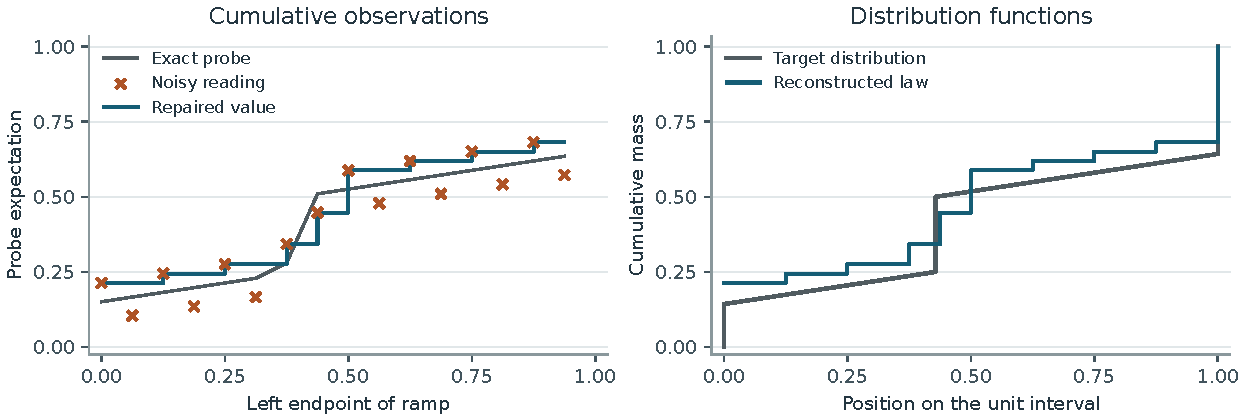
\includegraphics[width=.98\linewidth]{figures/ramp-repair.pdf}
\end{center}
The repair operates on cumulative ramp expectations. Their successive
differences define the atoms of the reconstructed law. The target's jumps at
$0,3/7,1$ are all admitted by the reconstruction theorem.

\subsection{Making the induction first-order}

The expression $\sum_i d_i L(B_i)$ in the proof abbreviates a finite
calculation. Here is a direct expansion which avoids induction on a statement
about arbitrarily many named scalars. Write $d_i=f(x_i)-f(x_{i+1})$ and
$S_0=f(x_N)\mathbf 1$, $S_{j+1}=S_j+d_j B_j$. Fix $r,t,n,f$ before
induction. The input's affine contract gives the rational inequality
\[
 |A(S_{j+1},t)-A(S_j,t)-d_jA(B_j,t)|\le(2+|d_j|)e_t.
\]
Telescope with induction on the cleared signed numerators, starting from
$|A(S_0,t)-f(x_N)|\le e_t$ by normalization and rational linearity with
auxiliary slack eliminated. The discrepancy between $A(S_N,t)$ and
$f(x_N)+\sum_{i<N}d_i A(B_i,t)$ is at most $(1+2N+K)e_t$.
For the prefix claim fix target index $i$ and use the upper bound
$A(B_i,t)+e_t+e_r$ for each of the first $i+1$ clipped samples.
Monotonicity of the true probes gives this finite bound by the rational
slack rule. The latest sample gives the converse lower bound with the same
slack. Both conclusions are inequalities between rationals. Letting the
auxiliary $t$ have enough bits for the final comparison recovers the displayed
constants. The proof can use finer readings than the law producer; those
readings do not enter its query budget.

\texttt{lean/PrefixObject.lean} defines the prefix accumulator as an actual
binary PR symbol parameterized by the syntactic body of a sample. It proves
inside the object calculus that the accumulator increases, covers the current
sample, and is bounded at a variable length $N$ by any common upper bound for
the first $N$ samples. Its induction matrix is
$i\le N\Rightarrow\mathrm{prefix}(i,x)\le u$. To use an integer upper bound,
multiply the finitely many positive denominators, including that of $u$, and
scale the clipped samples before applying the lemma. When a proposed upper
bound is negative the premises with any nonnegative sample give a finite
contradiction; empty prefixes have bound zero whenever $u\ge0$.
The signed Abel identity and construction of an attaining test are checked
in ambient Lean in \texttt{lean/LineDual.lean}.

\subsection{What becomes computable, and what still needs information}

\paragraph{Beyond Lipschitz tests.}
A rational-point evaluator for a continuous $g$ with a supplied modulus
$\omega$ satisfying $|x-y|\le2^{-\omega(k)}\Rightarrow |g(x)-g(y)|\le e_k$
gives a polygonal surrogate. Use mesh $2^{-\omega(p+2)}$, read its nodal
values with error $e_{p+2}$, and interpolate. Convexity of interpolation
bounds the uniform error by $2e_{p+2}$. Evaluate the resulting polygon
under the law presentation to accuracy $e_{p+1}$. The sum is at most $e_p$.
To compare two such estimates, apply the functional norm bound to their
polygons on a common refined grid. Thus the functional extends constructively
to all functions with this presentation. A Borel probability on the usual
unit interval yields such a functional semantically; the arithmetic
construction uses only its numerical input. No assertion about all subsets of
the interval is needed.

\paragraph{A discontinuous question about the law.}
Fix rational $0<t<1$. The map taking a law to its mass in $[0,t]$ cannot
have a continuous realizer on all these names. The laws $\delta_t$ and
$\delta_{t+s}$ have $W=s$ and give answers $1$ and $0$ whenever
$0<s\le1-t$. More directly, run a proposed finite reader at precision two on
the constant name $\delta_t$. For any finite set of indices read, pick
positive rational $s$ smaller than their radii and $1-t$.
A name can agree on those observations and use $\delta_{t+s}$ everywhere
else; its regularity follows from $W=s$. The same output cannot be within
$1/4$ of both answers.

A positive replacement is available given a rational width $\eta(p)>0$ at
which the mass in $(t-\eta,t+\eta)$ is bounded by $e_{p+2}$, with a
checkable presentation of this premise. Use lower and upper rational ramps
$g^-,g^+$ that go from $1$ to $0$ on $[t-\eta,t]$ and $[t,t+\eta]$,
restricted to $[0,1]$. They bracket the indicator and their difference vanishes
outside the open interval. An entirely numerical version of the premise
is $0\le L(g^+-g^-)\le e_{p+2}$. Evaluate the two polygonal tests within
$e_{p+2}$ and enlarge the resulting endpoints by $e_{p+2}$. This encloses
the desired value in a rational interval of width at most $5e_{p+2}$;
its midpoint has error at most $5e_{p+2}/2<e_p$. Even without a background
measure these midpoints are coherent: every lower ramp is bounded by every
upper ramp, so any two certified intervals overlap. The coherence estimate
then follows by adding the two radii. This specifies exactly what extra
information recovers the discontinuous observable.

Finally, an optimal coupling certifies distance between \emph{laws}. If a
prior application needs two random variables on a specified joint space,
the marginals do not determine their dependence. Two fair bits can be equal
almost surely or opposite almost surely with the same marginals. The
construction above supplies one joint realization for transport and Lipschitz
expectations. It preserves an already prescribed joint law only when additional
compatibility evidence is given.

\section{Changing the domain and composing the constructions}
\label{sec:transfer}

\subsection{A finite partition theorem on metric spaces}

The cumulative probes exploit order on the line. A simpler reconstruction
works on any bounded rational presentation with an explicitly supplied
partition of unity. This gives a comparison for the precision saved by the
one-dimensional construction and identifies the data needed on a new domain.

Let $D$ be a rational metric basis of diameter at most $H>0$, and let an
extensional test language contain constants, rational linear combinations and
the following supplied test functions. At level $n$ produce a nonempty list of
sites $x_1,\ldots,x_m$ and nonnegative tests $\psi_i$ with
$\sum_i\psi_i=1$ and $\psi_i(x)>0\Rightarrow d(x,x_i)\le h_n$.
Both the producer and the support and partition proofs are input contracts.
Assume also that the language contains the functions
$\min_i(v_i+d(x,x_i))$ for finite rational lists of sites and ordinates.
Distance evaluations and the displayed test constructors must be PR on basis
codes. Order claims about tests are proved pointwise on the dense basis.
In particular the positivity rule for $L$ applies to such proved comparisons.
Use a supplied schedule making $h_n$ small. If $L$ is presented on a smaller
test language, the additional constructors and their properties are obligations.

\begin{theorem}[Reconstruction from a partition]
Given a positive normalized rational-linear evaluator $L$, read each
$L(\psi_i)$ with error $\delta=2^{-r}$, where $m\delta\le1/2$.
In $O(m)$ rational operations after the oracle calls one can produce a
finite probability law $P$ on the sites satisfying
\[
             |P(f)-L(f)|\le K(h_n+Hm\delta)
\]
for every admitted $K$-Lipschitz test $f$. There is a PR procedure to compute
the maximum discrepancy of two finite laws against all 1-Lipschitz tests
in this language.
\end{theorem}
\begin{proof}
Write $c_i=L(\psi_i)$. Truncate negative readings to zero to obtain rational
$a_i$ with $|a_i-c_i|\le\delta$, and set $s=\sum_i a_i$.
Normalization and linearity give $|s-1|\le m\delta$. In particular
$s\ge1/2$. Set $P_i=a_i/s$. The sum of the normalization corrections
$\sum_i|P_i-a_i|$ is $|1-s|$. Thus $\sum_i|P_i-c_i|\le2m\delta$.
Here absolute values on named scalars can equally be evaluated by the regular
absolute-value operation. For an argument using only rational sign tests,
compare to arbitrary rational approximants to the $c_i$ and remove the
accumulated slack as in Section~\ref{sec:laws}.

The positive interpolant $Tf=\sum_i f(x_i)\psi_i$ approximates $f$ within
$Kh_n$ on the basis. Indeed its terms have nonnegative weights summing to
one and the support condition bounds every nonzero discrepancy. This can also
be proved without deciding equality of a named weight: check strict failure
of the rational distance test; in that case nonnegative $\psi_i$ with no
positive evidence is zero by the rational gap rule. Subtract the midpoint of
the greatest and least of the rational nodal ordinates when $f$ is a rational
test on the given sites. The deviations at the sites are at most $KH/2$,
and subtracting a constant leaves the mass discrepancy unchanged. This
proves the bound on replacing $c_i$ by $P_i$. For named nodal values choose rational $u_i$ within $e$ and use the admitted test $T_u=\sum_i u_i\psi_i$. Its uniform discrepancy from $f$ is at most $Kh_n+e$. Centering the rational ordinates bounds their magnitude by $KH/2+e$, and replacing the target ordinates in $P(f)$ adds at most $e$. Remove the resulting slack by the rational gap rule. Only the rational masses enter the producer.

Here is an explicit procedure for the second assertion. On the union of the
two supports fix a base vertex and normalize a potential to zero there.
Let $B$ be a common positive denominator for all pairwise distances. Enumerate
integer ordinates $v_i$ bounded in magnitude by $\lceil BH\rceil$, with
$v_0=0$ and $|v_i-v_j|\le B d(x_i,x_j)$. Return the largest signed score
of the ordinates $v_i/B$ against the difference of the masses. Each array
extends with these same nodal values by the finite minimum stipulated above.
This test is 1-Lipschitz by the triangle inequality.

For completeness of the search, start with any normalized \emph{rational}
feasible array $y$. For $0\le t<1$ set $v_i(t)=\lfloor B y_i+t\rfloor$.
Because $Bd(x_i,x_j)$ is an integer, these rounded arrays are still feasible,
and $v_0(t)=0$. The average of $v_i(t)$ over $t$ is $B y_i$, as one sees
by splitting at the single jump of that coordinate. Refinement by all jump
locations expresses the original score as a finite rational convex combination
of enumerated scores. The largest score dominates this combination. For a
test with named nodal values, the inequality follows by approximation: choose
rational approximations $u_i$ within $e$ and use the rational potential
$y_j=\min_i(u_i+d(x_i,x_j))$. It is feasible and within $e$ of the original
at each site. Normalize at the base vertex; the constant cancels, and the
score error is at most $2e$. Remove this slack. Reversing the test's sign
also bounds the absolute discrepancy.
\end{proof}

After merging zero-distance sites it is a metric: to detect a mass discrepancy at a single site, give that site the positive value of its least distance to the other sites and give all other sites value zero. The extension above is feasible. A support with one site has only one unit law. This test distance yields a regular law name by the same maximizing-test
two-run argument as on the line. Refine until $h_n\le2^{-p-1}$ and
$Hm\delta\le2^{-p-1}$, keeping $m\delta\le1/2$. The finite dual
enumeration is a decidability proof and a general algorithm; its worst-case
search size is exponential in the support size even for a fixed ordinate
range greater than one. The ordered scan in Lemma~\ref{lem:dual} removes
this search on the line and supplies a sparse primal coupling there.
The theorem above establishes a metric of continuous tests directly.

For example, on $[0,1]^d$ in the maximum distance use tensor products of
ordinary linear hats on the dyadic grid. Their products are nonnegative,
sum to one by multiplying the $d$ one-dimensional identities, and are
supported within one mesh step. With fixed precision $n$, $m=(2^n+1)^d$,
$H=1$ and $h_n=2^{-n}$. Rational piecewise polynomial tests with min and
max constructors suffice for these expressions; witnesses of positivity
can be hypotheses or explicit algebraic proofs. This instance needs no
general positivity decider for all expressions. For this simple normalization
method the required raw query precision grows as $\lceil\log_2 m\rceil$.
On $[0,1]$, Section~\ref{sec:laws} eliminates that term by probing the
cumulative sums directly.

\subsection{A quantile from a transport name}

The operator for roots accepts a general function evaluator. The law
construction can provide it, even though a distribution function at an
atom was a counterexample. Suppose now the inputs have the following density bounds on rational test functions
\[
 2^{-b}\int_0^1 h\ \le L(h)\le 2^d\int_0^1 h
 \qquad(0\le h\in\PL)
\]
with supplied integers $b,d$. Every displayed polygonal integral is a finite
rational trapezoid sum. For a rational $x\in[0,1]$ let $R_{x,\eta}$ be the
right ramp of width $\eta$, equal to one through $x$ and zero past $x+\eta$,
restricted to $[0,1]$. Its area lies between $x$ and $x+\eta$. At fixed
$x$ the ramps are ordered by width. The upper density bound shows that the
two expectations at widths $\eta,\eta'$ differ by at most
$2^d\max(\eta,\eta')$. Thus they define a scalar $C(x)$ and the error at
one width is at most $2^d\eta$. For $y\ge x$ the difference of the two
equal-width ramps is nonnegative and its integral tends to $y-x$ with
error at most $\eta$. Applying both density comparisons to that difference
and removing the auxiliary width proves
\[
 2^{-b}(y-x)\le C(y)-C(x)\le2^d(y-x).
\]
The resulting function has endpoint values $C(0)=0,C(1)=1$. With
a semantic probability measure, $C$ is its distribution function.

Given a law name $M$, to evaluate $C(x)$ at precision $p$ use
$\eta=2^{-(p+d+2)}$ and the single finite law at level $\ell=2p+d+4$.
The ramp has Lipschitz constant at most $1/\eta$. Its value under $M_\ell$
has discrepancy at most $2^{-\ell}/\eta=e_p/4$ from $L(R_{x,\eta})$.
The width error is also at most $e_p/4$. Both estimates include $x=0,1$.
Subtract a rational target mass $\alpha\in[0,1]$ to obtain observations
for Section~\ref{sec:conditioned-zero} with $g(k)=k+b$ and $\mu(k)=k+d$.
Consequently one finite-law observation per halving produces a coherent name
for the unique $\alpha$-quantile. At halving $j$ its level is
$2(j+b+3)+d+4$. This counts law observations. The number of atoms encoded
by one observed law still affects the work to integrate the ramp. The upper
density promise supplies a CDF evaluator; the lower promise supplies the
inverse modulus. Their roles are distinct. The construction feeds its
explicit moduli through the general composition rule instead of taking an
inverse of a black-box distribution function.


For an exact instance, take density $1/2+x$ on $[0,1]$. Here $b=d=1$
suffice, and the distribution function for independent checking is
$(x+x^2)/2$. The program \texttt{examples/quantiles.py} represents the
level-$\ell$ law by moving each dyadic cell's mass to its left endpoint.
This costs at most $2^{-\ell}$. It sums a ramp on this law from the first
two prefix moments, so it can use very fine levels without materializing the
grid. At $\alpha=7/15$, 32 calls give the bracket
$[5049260259,5049260261]/8589934592$. Substitution in the quadratic verifies
the inequalities at both endpoints. The program also exercises $\alpha=0$
and $\alpha=1$, and checks the compressed evaluation against direct finite sums.

\section{Proof status, reproduction, and further questions}
\label{sec:replay}

\subsection{What Lean checks}

\noindent\begin{tabularx}{\linewidth}{@{}p{.23\linewidth}YY@{}}
\toprule
Component & Kernel-checked result & Remaining object derivation\\
\midrule
Finite observations & Object iPRA sparse replay at variable time. Lean window certification, composition of prefix dependence and no-window example. & Reify the field operations for each reader and prove its finite use and extensionality contracts.\\[3pt]
Zero selection & Lean brackets, dyadic widths, cross-stage midpoint bound and residual schedule. Closed iPRA theorem for the three sign branches. & Compile the dyadic transition and run the stage induction at fixed test precision.\\[3pt]
Differentiation & Lean local signed bounds. Closed iPRA theorem deriving both child/parent comparisons from the adjacent-child comparison. & Sum the errors over a level path, derive the cell estimates, apply the tagged FTC and pass to the names.\\[3pt]
Interval laws & Lean finite Abel formula and optimal dual potential. Object iPRA variable-length prefix maximum and its common upper bound. & Code the sparse coupling and verify the two marginal scans and reconstruction contracts.\\[3pt]
Metric partitions and quantiles & Human proofs and explicit programs or finite bounds. Exact-arithmetic regression for the density $1/2+x$. & Reify rounding of finite potentials and compose the ramp accuracy proof with the midpoint invariant.\\
\bottomrule
\end{tabularx}

The archive contains four standalone Lean modules using the Lean 4.32 standard
distribution, and four modules importing ProveIt. In the latter, the exported
types mention \texttt{Prf PRAAx} literally. The zero and slope lemmas close
their seven numerical variables in the object language. The prefix scan is
a derivation constructor at arbitrary terms and hypotheses with the raw sample
body fixed syntactically. Sparse replay has the same schema form for fixed reader instructions. All four use intuitionistic object rules. The
ordinary Lean metatheory used by the upstream proof infrastructure reports
\texttt{propext}, \texttt{Classical.choice}, and \texttt{Quot.sound} for the
audited object results. These constants occur in the host implementation of
proof constructions. The object judgments use the repository's intuitionistic axiom family.

\subsection{Dependency order for completing the formalization}

\begin{enumerate}[leftmargin=*]
\item Define a total encoding of lists, reduced dyadic sites and signed
rationals on top of \texttt{PTm.toPR}, \texttt{recDef} and the pairing and
order modules. Prove normalization preserves equality and cross-multiplication
comparison, addition, multiplication, absolute value and clipping. A unit
interval site may be coded by numerator and power-of-two denominator with a
clipping operation. Record validity checks for arbitrary input codes. Fix input
evaluator symbols and numerical parameters when forming a sequent.
\item Formalize regularity, point equality, forward and inverse moduli, and
value-table inequalities as universally closed formulas with the rational
operations expanded. For instance, the slope contract for $A,b$ quantifies
over the natural triple $(n,j,p)$ and, under $0<j<2^n$, tests the two signed
cross-multiplied versions of \eqref{eq:dd-grid}. Trace verification and legality
of queries use bounded scans. For a fixed reader, substitute a PR symbol for
each transition and apply the checked sparse replay theorem to its two state codes at the requested terminal slot.
\item For the roots, prove the two defining equations of the integer endpoint
recurrence, instantiate the checked three-way sequent and use the width and
sign invariants at fixed outer precision. At a single final precision choose
the starting stage from $\mu$ and finish with \eqref{eq:zero-forward}.
For differentiation use the ancestor-induction and slack bounds beside
\eqref{eq:dd-finite}. Prove the signed cell estimate before using the
repository's tagged-sum derivations. Its two bounds have hypotheses for every
cell, so the passage must include the denominator scale for each finite
tagged term and both endpoints. A product of the finite denominators is a
sufficient common positive scale.
\item For laws, code mergers and residual atom weights by the integer
numerators at a common positive denominator. At each transfer maintain the
two prescribed masses less the emitted row and column sums. Transfer their
minimum and advance at least one cursor. The sum of the remaining numbers of
sites decreases; iteration for $s+t$ steps with an absorbing final state
is PR. At a fixed cut maintain the cumulative crossing flow and use the common
mass-coordinate formula of Lemma~\ref{lem:dual}. Use the repository's
\texttt{Sums.abel\_summation} for the signed equality after denominator
clearing, splitting signed terms into their natural components. The finite
host specification checks the index and boundary conventions.
\item Apply \texttt{prefix\_upper} at length $i+1$ to the repaired ramp readings.
Derive the lower bound using \texttt{covers\_latest}. Prove the prefix
expansion of the interpolant at fixed auxiliary precision as in
Section~\ref{sec:laws}, then instantiate the maximizing polygon constructed
from the two outputs. For a new partition language reify its constructor
identities (in particular the sum of the weights), the support comparison and
finite minimum extension. A dyadic cube uses bounded products of $d$ hats.
For finite dual search enumerate the bounded ordinate array, sort its
fractional jumps, and telescope the positive rational layer lengths. This
supplies the selection proof for the finite maximum. For the quantile
specialize the law evaluator to the right ramp with the displayed level
$2p+d+4$, weaken the input and output estimates to the root contracts,
and apply the signed stage induction from step 3.
\end{enumerate}
These steps specify the inputs to each open lemma, the bounded witness, the
induction matrix or its rational inequality, and the existing module it uses.
The full operators currently have human arithmetic proofs and partially
mechanized components.

\subsection{Sources and further research}

The source inventory accompanying the paper records the pinned repository
paths. The main external references are
A. Pauly, \emph{On the topological aspects of the theory of represented
spaces} (2016), \href{https://arxiv.org/abs/1204.3763}{author preprint};
A. Kawamura and S. Cook, \emph{Complexity theory for operators in analysis},
\href{https://arxiv.org/abs/1305.0453}{author preprint};
M. Hoyrup and C. Rojas, \emph{Computability of probability measures and
Martin-L\"of randomness over metric spaces} (2009),
\href{https://doi.org/10.1016/j.ic.2008.12.009}{published paper}; and
S. S. Vallander, \emph{Calculation of the Wasserstein distance between
probability distributions on the line} (1973, English translation 1974),
\href{https://doi.org/10.1137/1118101}{published paper}.
The one-dimensional transport formula is classical in this literature. Its
use here supplies finite certificates and precision schedules for an
iPRA representation change.

\begin{itemize}
\item On a metric tree, deleting an edge separates the sites into two
components. Can subtree probes replace the line's cumulative ramps and allow
precision to depend on weighted branch length in place of the total number
of cells?
\item Can the dyadic second-difference test use locally varying tail certificates
to construct derivatives on certified subintervals? At a shared endpoint the
two one-sided slope bounds must still give a compatible value.
\item For structured finite laws, which mesh and mass queries can be shared
between successive quantile bits? The worked example uses prefix moments.
A general adaptive version needs a verifiable bound on the cost of each
compressed query and a proof that it realizes the declared finite law.
\end{itemize}

\end{document}
